% STATUS: ACTIVE -- first-order gain model: Kalman filter, two tracks, y2 only with Q44 = 0 -> weighted average -> three cases.
% ======================================================
% Compile: xelatex 0929_kf_two_tracks.tex   (from reference/eq17_analysis/derivation/)
% Notation: model and symbols from 0927_obs_first_order_v1.tex; Kalman filter notation and order from
%   Meng 2025 near-wall paper, Sec. II.F (L[k], P^f[k], P[k]; estimate at k+1 from errors at k).
% Sections: 1 model | 2 estimator and Kalman filter | 3 two tracks | 4 y2 only, Q44 = 0: weighted average |
%   figure page for 4.7 | 5 y1 added.
% Checked numerically (tmp chk_kf.py / splice.py, 2026-09-29): l41, l42, the exact 1/P_aa of 5.3, 4.5 with varying R2.
% Figure: fig_noap_y2_average_td5_td50.png (test_script/scratch/plot_5state_noap_y2_average.m, y2 weights = diag.w_y2).
% Equations only (derivation-workflow rule 10).
% ======================================================
\documentclass[11pt,a4paper]{ctexart}
\usepackage[fleqn]{amsmath}
\usepackage{amssymb,bm}
\usepackage{graphicx}
\graphicspath{{figures/}}
\setlength{\mathindent}{0pt}
\usepackage{geometry}
\geometry{margin=2.2cm}
\setlength{\parindent}{0pt}
\setlength{\parskip}{0.2em}
\setlength{\abovedisplayskip}{6pt}
\setlength{\belowdisplayskip}{6pt}
\setlength{\abovedisplayshortskip}{6pt}
\setlength{\belowdisplayshortskip}{6pt}
\newcommand{\lc}{\lambda_c}
\newcommand{\hd}[1]{\par\bigskip\noindent\underline{\textbf{#1}}}
\pagestyle{plain}

\begin{document}

\begin{center}\textbf{\large First-order gain model: Kalman filter, $y_2$ only, the estimate as a weighted average}\end{center}

%======================================================================
\section{Model}

\hd{State equation}
\[
\begin{aligned}
\delta x_1[k+1] &= \delta x_2[k] \\
\delta x_2[k+1] &= \delta x_3[k] \\
\delta x_3[k+1] &= \lc \cdot \delta x_3[k] - F_{dx}[k]\cdot e_{a_x}[k] - \varepsilon[k] \\
a_x[k+1] &= a_x[k]
\end{aligned}
\]
\[
F_{dx}[k] = f_{dx}[k] + (1-\lc)\textstyle\sum_{i=1}^{d} f_{dx}[k-i] \;\approx\; \big(1 + (1-\lc)d\big)\,\dfrac{\Delta x_d[k]}{\hat a_x[k]} \qquad (\text{constant velocity})
\]

\hd{Output equation}
\[
\begin{aligned}
y_1[k] &= \delta x_1[k] + n_x[k], \qquad R_1 = \mathrm{Var}(n_x) \\
y_2[k] &= a_x[k] + n_a[k], \qquad\;\; R_2[k] = \mathrm{Var}(n_a[k])
\end{aligned}
\]

\hd{Estimation error and output error}
\[
\mathbf{e}[k] = \begin{bmatrix} e_{\delta x_1}[k] \\ e_{\delta x_2}[k] \\ e_{\delta x_3}[k] \\ e_{a_x}[k] \end{bmatrix}
= \begin{bmatrix} \delta x_1[k] - \delta\hat x_1[k] \\ \delta x_2[k] - \delta\hat x_2[k] \\ \delta x_3[k] - \delta\hat x_3[k] \\ a_x[k] - \hat a_x[k] \end{bmatrix},
\qquad
\begin{aligned}
e_{y_1}[k] &= y_1[k] - \delta\hat x_1[k] = e_{\delta x_1}[k] + n_x[k] \\
e_{y_2}[k] &= y_2[k] - \hat a_x[k] = e_{a_x}[k] + n_a[k]
\end{aligned}
\]

\hd{Matrices}
\[
\mathbf{F}_e[k] =
\begin{bmatrix}
0 & 1 & 0 & 0 \\
0 & 0 & 1 & 0 \\
0 & 0 & \lc & -F_{dx}[k] \\
0 & 0 & 0 & 1
\end{bmatrix},
\qquad
\mathbf{H} =
\begin{bmatrix}
1 & 0 & 0 & 0 \\
0 & 0 & 0 & 1
\end{bmatrix}
\]
\[
\mathbf{Q} = \mathrm{diag}(0,\, 0,\, Q_{33},\, Q_{44}),
\qquad
\mathbf{R}[k] = \mathrm{diag}(R_1,\, R_2[k]),
\qquad
\text{first order: } Q_{44} = 0
\]

%======================================================================
\clearpage
\section{Estimator and Kalman filter}

\hd{2.1 Estimator (model one step ahead, plus gain times output error)}
\[
\begin{aligned}
\delta\hat x_1[k+1] &= \delta\hat x_2[k] + \ell_{21}[k]\,e_{y_1}[k] + \ell_{22}[k]\,e_{y_2}[k] \\
\delta\hat x_2[k+1] &= \delta\hat x_3[k] + \ell_{31}[k]\,e_{y_1}[k] + \ell_{32}[k]\,e_{y_2}[k] \\
\delta\hat x_3[k+1] &= \lc\,\delta\hat x_3[k] + \big(\lc\,\ell_{31}[k] - F_{dx}[k]\,\ell_{41}[k]\big)\,e_{y_1}[k] + \big(\lc\,\ell_{32}[k] - F_{dx}[k]\,\ell_{42}[k]\big)\,e_{y_2}[k] \\
\hat a_x[k+1] &= \hat a_x[k] + \ell_{41}[k]\,e_{y_1}[k] + \ell_{42}[k]\,e_{y_2}[k]
\end{aligned}
\]
\[
\mathbf{L}[k] = \begin{bmatrix}
\ell_{11}[k] & \ell_{12}[k] \\
\ell_{21}[k] & \ell_{22}[k] \\
\ell_{31}[k] & \ell_{32}[k] \\
\ell_{41}[k] & \ell_{42}[k]
\end{bmatrix}
\qquad (\text{row } i = \text{state } i, \quad \text{column } 1 = y_1, \quad \text{column } 2 = y_2)
\]

\hd{2.2 Error dynamics}
\[
\mathbf{e}[k+1] = \mathbf{F}_e[k]\,\big(\mathbf{I} - \mathbf{L}[k]\,\mathbf{H}\big)\,\mathbf{e}[k]
- \mathbf{F}_e[k]\,\mathbf{L}[k]\begin{bmatrix} n_x[k] \\ n_a[k] \end{bmatrix}
+ \begin{bmatrix} 0 \\ 0 \\ -\varepsilon[k] \\ 0 \end{bmatrix}
\]

\hd{2.3 Kalman filter (every step, in this order)}
\[
\begin{aligned}
\mathbf{L}[k] &= \mathbf{P}^f[k]\,\mathbf{H}^T\big(\mathbf{H}\,\mathbf{P}^f[k]\,\mathbf{H}^T + \mathbf{R}[k]\big)^{-1} \\
\mathbf{P}[k] &= \big(\mathbf{I} - \mathbf{L}[k]\,\mathbf{H}\big)\,\mathbf{P}^f[k] \\
\mathbf{P}^f[k+1] &= \mathbf{F}_e[k]\,\mathbf{P}[k]\,\mathbf{F}_e^T[k] + \mathbf{Q}
\end{aligned}
\]
\[
\mathbf{P}^f[k] = \mathrm{Cov}\big(\mathbf{e}[k]\big) \text{ before the readings of step } k, \qquad
\mathbf{P}[k] = \text{after them}, \qquad
\mathbf{P}^f[0] = \text{initial value}
\]

%======================================================================
\clearpage
\section{Two tracks}

\hd{3.1 Track 1: 2.3 (confidence and gain)}
\[
\mathbf{P}^f[0] \;\xrightarrow{\;\mathbf{F}_e,\ \mathbf{H},\ \mathbf{Q},\ \mathbf{R}\;}\;
\mathbf{L}[0],\ \mathbf{P}[0],\ \mathbf{P}^f[1] \;\longrightarrow\;
\mathbf{L}[1],\ \mathbf{P}[1],\ \mathbf{P}^f[2] \;\longrightarrow\; \cdots
\qquad (y_1,\ y_2 \text{ do not appear})
\]

\hd{3.2 Track 2: 2.1 (estimate)}
\[
\hat a_x[k] \;\xrightarrow{\;y_1[k],\ y_2[k]\ \text{through}\ e_{y_1}[k],\ e_{y_2}[k];\ \ \ell_{41}[k],\ \ell_{42}[k]\ \text{from track 1}\;}\; \hat a_x[k+1]
\]

\hd{3.3 Where the tracks touch}
\[
F_{dx}[k] \ni \hat a_x[k], \qquad Q_{33} \ni \hat a_x, \qquad R_2[k] \ni \hat a_x[k]
\qquad (\text{track 1 reads track 2 only through these})
\]

%======================================================================
\clearpage
\section{$y_2$ only, $Q_{44} = 0$: the gain row step by step}

\hd{4.1 2.3 with $\mathbf{H} = [\,0 \;\; 0 \;\; 0 \;\; 1\,]$, $\mathbf{R} = R_2[k]$ (the $a_x$ element)}
\[
\begin{aligned}
\ell_{42}[k] &= \frac{P^f_{aa}[k]}{P^f_{aa}[k] + R_2[k]} \\
P_{aa}[k] &= \big(1 - \ell_{42}[k]\big)\,P^f_{aa}[k] = \frac{R_2[k]\,P^f_{aa}[k]}{P^f_{aa}[k] + R_2[k]} \\
P^f_{aa}[k+1] &= P_{aa}[k] + Q_{44} = P_{aa}[k]
\end{aligned}
\]

\hd{4.2 2.1, the $a_x$ row}
\[
\begin{aligned}
\hat a_x[k+1] &= \hat a_x[k] + \ell_{42}[k]\,\big(y_2[k] - \hat a_x[k]\big) \\
&= \big(1 - \ell_{42}[k]\big)\,\hat a_x[k] + \ell_{42}[k]\,y_2[k]
\end{aligned}
\]

\hd{4.3 Substitute back, $k = 0, 1, 2$}
\[
\begin{aligned}
\hat a_x[1] &= (1-\ell_{42}[0])\,\hat a_x[0] + \ell_{42}[0]\,y_2[0] \\[0.8ex]
\hat a_x[2] &= (1-\ell_{42}[1])\,\hat a_x[1] + \ell_{42}[1]\,y_2[1] \\
&= (1-\ell_{42}[1])(1-\ell_{42}[0])\,\hat a_x[0] \\
&\quad + (1-\ell_{42}[1])\,\ell_{42}[0]\,y_2[0] \\
&\quad + \ell_{42}[1]\,y_2[1] \\[0.8ex]
\hat a_x[3] &= (1-\ell_{42}[2])\,\hat a_x[2] + \ell_{42}[2]\,y_2[2] \\
&= (1-\ell_{42}[2])(1-\ell_{42}[1])(1-\ell_{42}[0])\,\hat a_x[0] \\
&\quad + (1-\ell_{42}[2])(1-\ell_{42}[1])\,\ell_{42}[0]\,y_2[0] \\
&\quad + (1-\ell_{42}[2])\,\ell_{42}[1]\,y_2[1] \\
&\quad + \ell_{42}[2]\,y_2[2]
\end{aligned}
\]

\hd{4.4 General step $k$}
\[
\hat a_x[k] = \prod_{i=0}^{k-1}\big(1 - \ell_{42}[i]\big)\;\hat a_x[0] + \sum_{j=0}^{k-1} c_{k,j}\,y_2[j],
\qquad
c_{k,j} = \ell_{42}[j]\prod_{i=j+1}^{k-1}\big(1 - \ell_{42}[i]\big)
\]

%----------------------------------------------------------------------
\clearpage
\hd{4.5 The products telescope (4.1)}
\[
\begin{aligned}
1 - \ell_{42}[i] &= \frac{P_{aa}[i]}{P^f_{aa}[i]} = \frac{P^f_{aa}[i+1]}{P^f_{aa}[i]}, \qquad
\ell_{42}[j] = \frac{P^f_{aa}[j]}{P^f_{aa}[j] + R_2[j]} = \frac{P_{aa}[j]}{R_2[j]} \\
\prod_{i=j+1}^{k-1}\big(1 - \ell_{42}[i]\big) &= \frac{P^f_{aa}[j+2]}{P^f_{aa}[j+1]}\cdot\frac{P^f_{aa}[j+3]}{P^f_{aa}[j+2]}\cdots\frac{P^f_{aa}[k]}{P^f_{aa}[k-1]}
= \frac{P^f_{aa}[k]}{P^f_{aa}[j+1]} = \frac{P^f_{aa}[k]}{P_{aa}[j]} \\
c_{k,j} &= \frac{P_{aa}[j]}{R_2[j]}\cdot\frac{P^f_{aa}[k]}{P_{aa}[j]} = \frac{P^f_{aa}[k]}{R_2[j]} \\
\prod_{i=0}^{k-1}\big(1 - \ell_{42}[i]\big) &= \frac{P^f_{aa}[k]}{P^f_{aa}[0]} \\
\frac{1}{P^f_{aa}[k+1]} &= \frac{P^f_{aa}[k] + R_2[k]}{R_2[k]\,P^f_{aa}[k]} = \frac{1}{P^f_{aa}[k]} + \frac{1}{R_2[k]}
\;\Rightarrow\;
\frac{1}{P^f_{aa}[k]} = \frac{1}{P^f_{aa}[0]} + \sum_{j=0}^{k-1}\frac{1}{R_2[j]}
\end{aligned}
\]

\hd{4.6 The estimate is a weighted average of the readings}
\[
\boxed{\;
\hat a_x[k] = \frac{\dfrac{1}{P^f_{aa}[0]}\,\hat a_x[0] + \displaystyle\sum_{j=0}^{k-1}\frac{1}{R_2[j]}\,y_2[j]}{\dfrac{1}{P^f_{aa}[0]} + \displaystyle\sum_{j=0}^{k-1}\frac{1}{R_2[j]}}
\;}
\]
\[
R_2 \text{ constant: } \;
\hat a_x[k] = \frac{m\,\hat a_x[0] + \sum_{j=0}^{k-1} y_2[j]}{m + k}, \quad m = \frac{R_2}{P^f_{aa}[0]}
\]

\hd{4.7 Readings are true gain plus noise}
\[
y_2[j] = a_x[j] + n_a[j]
\;\Rightarrow\;
\hat a_x[k] = \frac{\dfrac{1}{P^f_{aa}[0]}\,\hat a_x[0] + \displaystyle\sum_{j=0}^{k-1}\frac{1}{R_2[j]}\,a_x[j]}{\dfrac{1}{P^f_{aa}[k]}}
+ \frac{\displaystyle\sum_{j=0}^{k-1}\frac{1}{R_2[j]}\,n_a[j]}{\dfrac{1}{P^f_{aa}[k]}}
\]

\clearpage
\section*{4.7: plane, 22.2 $\to$ 1.10 R in $T_d = 5$ s vs $50$ s, then hold; dashed = first term of 4.7 (initial estimate and true gains, weights $1/R_2[j]$)}
\begin{center}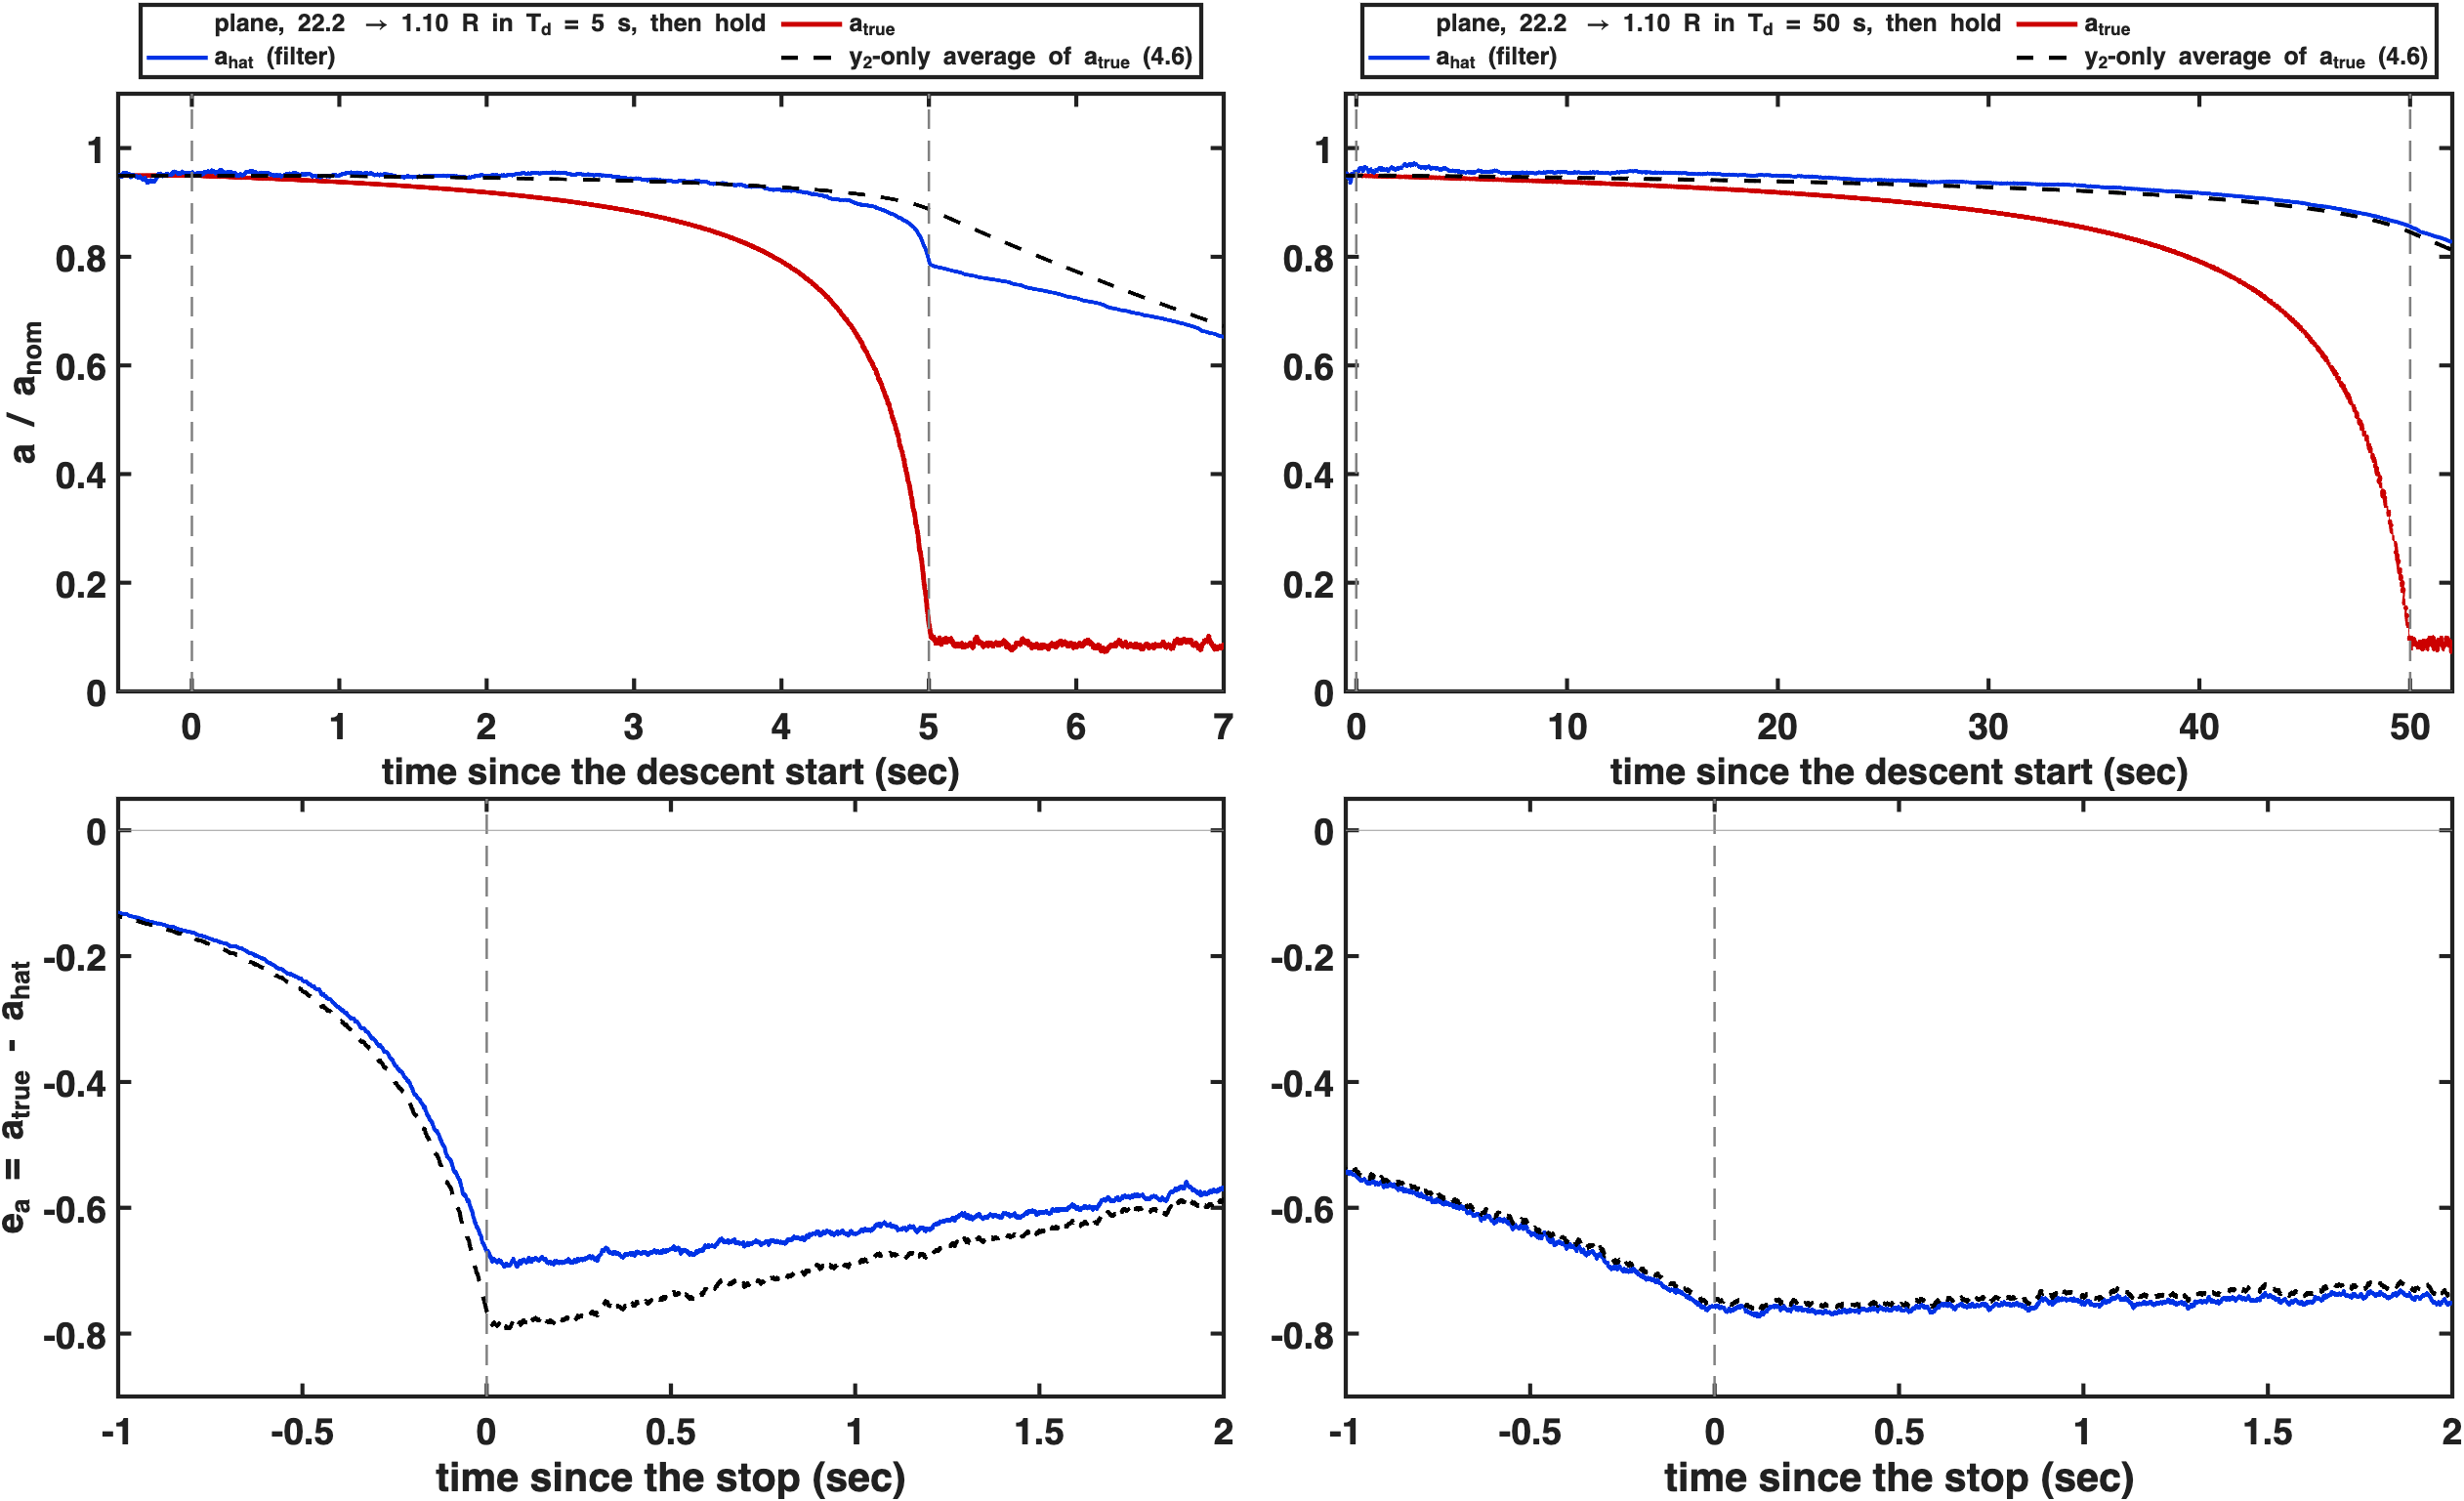
\includegraphics[width=\textwidth]{fig_noap_y2_average_td5_td50.png}\end{center}

%======================================================================
\clearpage
\section{$y_1$ added}

\hd{5.1 2.3, third line, the $a_x$ column of $\mathbf{P}^f$}
\[
\begin{aligned}
P^f_{1a}[k+1] &= P_{2a}[k] \\
P^f_{2a}[k+1] &= P_{3a}[k] \\
P^f_{3a}[k+1] &= \lc\,P_{3a}[k] - F_{dx}[k]\,P_{aa}[k]
\end{aligned}
\qquad\qquad
P^f_{1a} \;\to\; -\frac{F_{dx}}{1-\lc}\,P_{aa} \quad (F_{dx} \text{ constant})
\]

\hd{5.2 2.3, first line, both outputs}
\[
\begin{aligned}
D[k] &= \big(P^f_{11}[k] + R_1\big)\big(P^f_{aa}[k] + R_2[k]\big) - \big(P^f_{1a}[k]\big)^2 \\
\ell_{41}[k] &= \frac{P^f_{a1}[k]\,R_2[k]}{D[k]}, \qquad
\ell_{42}[k] = \frac{P^f_{aa}[k]\big(P^f_{11}[k] + R_1\big) - \big(P^f_{a1}[k]\big)^2}{D[k]}
\end{aligned}
\]

\hd{5.3 2.3, second line: the weight of one step}
\[
\begin{aligned}
\frac{1}{P_{aa}[k]} &= \frac{1}{P^f_{aa}[k]} + \frac{1}{R_2[k]}
+ \frac{\big(P^f_{1a}[k] / P^f_{aa}[k]\big)^2}{P^f_{11}[k] - \big(P^f_{1a}[k]\big)^2 / P^f_{aa}[k] + R_1} \\
&\approx \frac{1}{P^f_{aa}[k]} + \frac{1}{R_2[k]} + \frac{1}{P^f_{11}[k] + R_1}\left(\frac{F_{dx}[k]}{1-\lc}\right)^{2},
\qquad \frac{F_{dx}}{1-\lc} \propto \frac{\Delta x_d}{\hat a_x} \propto \frac{1}{T_d\,\hat a_x}
\end{aligned}
\]

\end{document}
